\documentclass{article}

\usepackage{arxiv}
\usepackage{lineno} % line numbers
\usepackage{lipsum} % placeholder text
\usepackage{graphicx} % figures path
\usepackage{authblk} % author block
\usepackage{hyperref} 
\usepackage[labelfont=bf]{caption} 

\usepackage{newfloat}
\DeclareFloatingEnvironment[name={Supplementary Table},fileext=lst,listname={List of 
Supplementary Tables}]{supptable}
\DeclareFloatingEnvironment[name={Supplementary Figure},fileext=lsf,listname={List of Supplementary Figures}]{suppfigure}

\graphicspath{./figures/}

\linenumbers % add line numbers
\raggedbottom % removes vbox warning
% to have the ending sections sepparate
\def\backmatter{
    \setcounter{section}{0}
    \renewcommand{\thesection}{\Alph{section}}
}

\title{
    My title
}

%%%%%%%%%%%%%%%  Author list  %%%%%%%%%%%%%%%%%%%%%%%%%%%%%%%%%%%%%%%%%%%%%%%%%%

\author[1,2,\thanks{These authors contributted equally}]{Alice Smith}
\author[2,$^*$]{John doe}
\author[2,\thanks{Correspondence: \tt{bjones@college.edu}}]{Bob Jones}

\affil[1]{Department of Mathematics, University X}
\affil[2]{Department of Biology, University Y}

%%%%%%%%%%%%%%%  Author list  %%%%%%%%%%%%%%%%%%%%%%%%%%%%%%%%%%%%%%%%%%%%%%%%%%

\begin{document}

\maketitle

\begin{abstract}
\lipsum[1-1]
\end{abstract}
    
    
% keywords can be removed
\keywords{
    Keyword1 
    \and 
    Keyword2
    \and 
    Keyword3 
    \and 
    Keyword4
}

\section*{Introduction}

\lipsum[1-5]

\section*{Results}

\subsection*{First results}

\lipsum[1-1]

\begin{figure}[h]
    \centering
    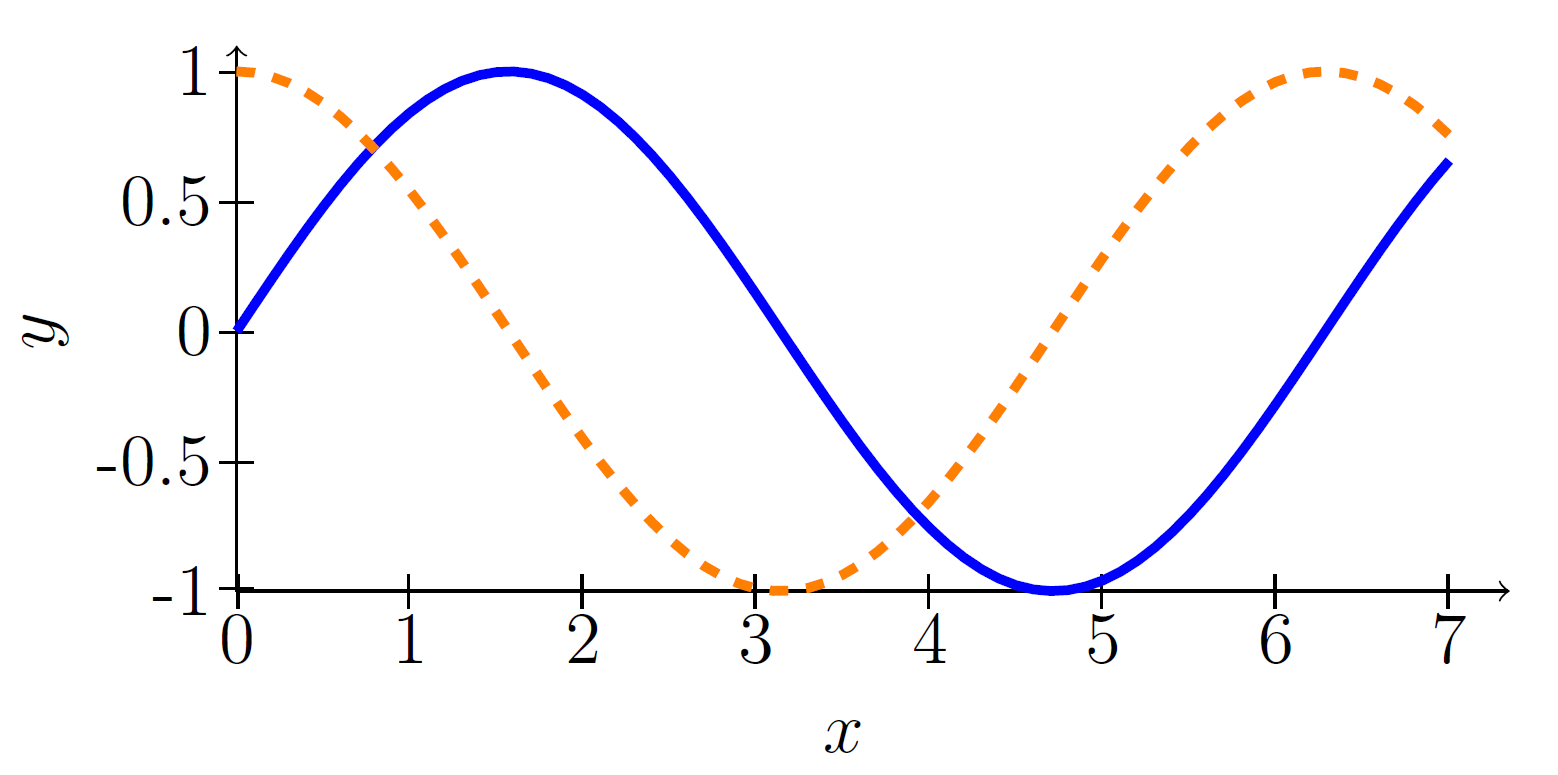
\includegraphics[width=0.5\textwidth]{figures/fig1.png}
    \caption{My figure}
\end{figure}

\subsection*{Second results}

\lipsum[1-1]

\section*{Discussion}

\lipsum[1-2]

\section*{Methods}

\subsection*{First methods}

\lipsum[1-1]

\subsection*{Second methods}

\lipsum[1-1]

%%%%%%%%%%%%%%%%%%%%%%%%%%%%%%%%%%%%%%%%%%%%%%%%%%%%%%%%%%%%%%%%%%%%%%%%%%%%%%%%
%%                                          
%% Backmatter begins here                   
%%                                          
%% Here are additional sections to the paper, add/remove them as required
%%                                          
%%%%%%%%%%%%%%%%%%%%%%%%%%%%%%%%%%%%%%%%%%%%%%%%%%%%%%%%%%%%%%%%%%%%%%%%%%%%%%%%

\begin{backmatter}

\section*{Abbreviations}
\begin{itemize}
    \item A - Adenine
\end{itemize}
    
\section*{Availability of data and materials}
Write if applicable.

\section*{Acknowledgements}
Write if applicable.

\section*{Funding}
Write if applicable.

\section*{Ethics approval and consent to participate}
Write if applicable.

\section*{Competing interests}
Write if applicable.

\section*{Consent for publication}
Write if applicable.
    
\section*{Authors' contributions}
Write if applicable.

\section*{Supplemental material}
\begin{itemize}
    \item Filename.ext - Description of the file contents.
\end{itemize}

\end{backmatter}

\newpage
\setcounter{page}{1}
\setcounter{linenumber}{1}
\listofsuppfigures
%\listofsupptables
\newpage

\begin{suppfigure}[ht!]
    \centering
    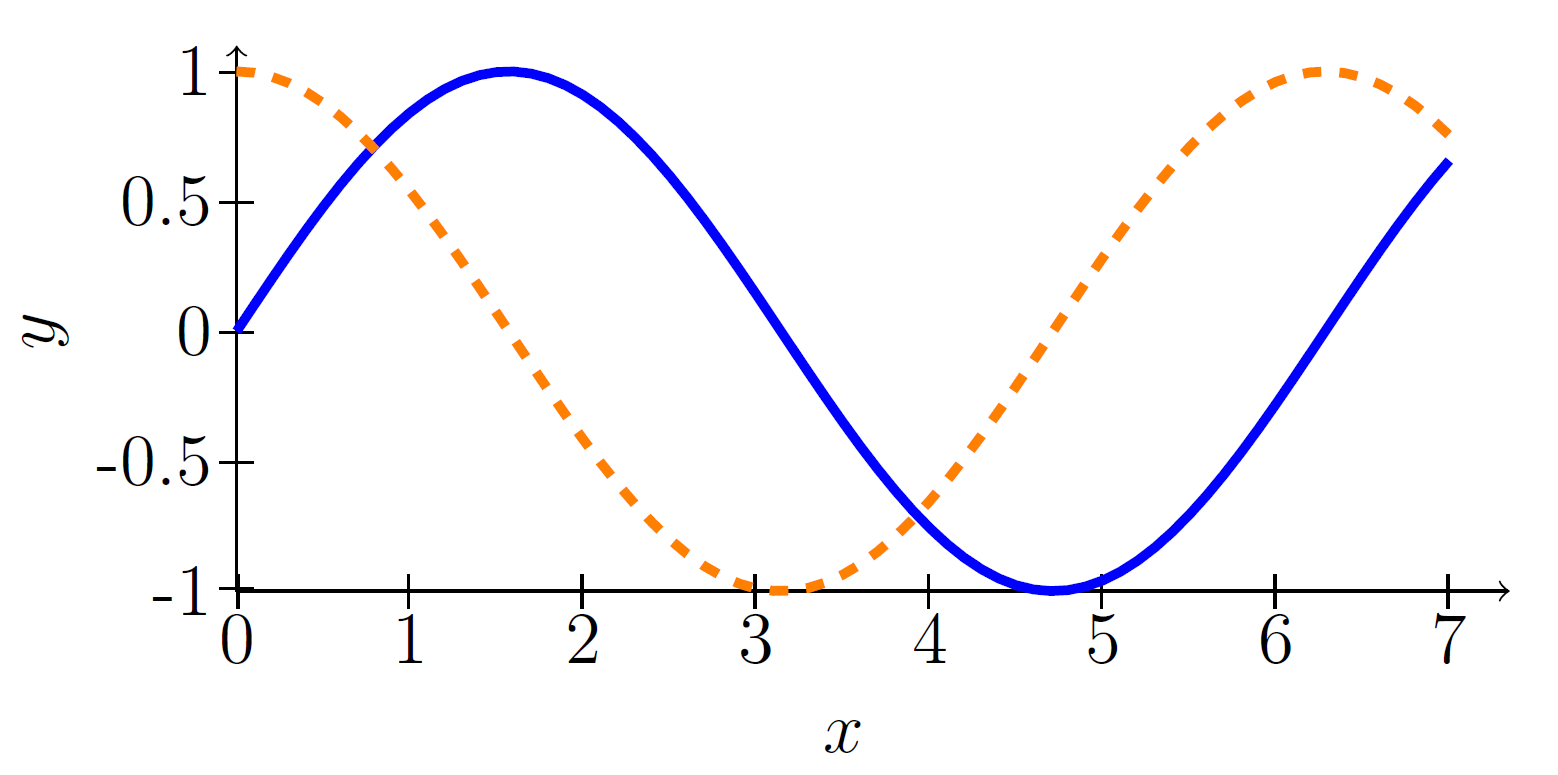
\includegraphics[scale=0.10]{figures/supfig1.png}
    \caption{Summary of dataset sizes}
    {Number of reads per dataset that were successfully resquiggled (blue) or that failed (orange).}
\end{suppfigure}

\end{document}